Finden Sie die kritischen Punkte von 
\begin{equation}
\frac{d}{dx}\begin{pmatrix}y_1\\y_2\end{pmatrix}
=
\begin{pmatrix}
y_2\\
-y_2+\alpha(y_1^2-1)
\end{pmatrix}
\label{603:dgl}
\end{equation}
mit $\alpha > \frac18$, und diskutieren Sie deren Stabilit"at.

\begin{loesung}
\begin{figure}
\centering
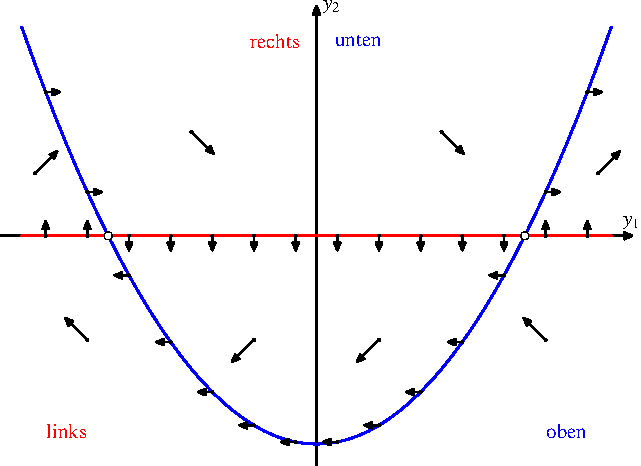
\includegraphics{../skript/uebungsaufgaben/603-1.pdf}
\caption{Nullklinen des Differentialgleichungssystems~(\ref{603:dgl})
mit $\alpha=1$
\label{603:nullklinen}}
\end{figure}
Wir bestimmen die Nullklinen.
Die $y_1$-Nullkline ist die $y_1$-Achse mit der Gleichung $y_2=0$.
die $y_2$-Nullkline erf"ullt die Gleichung
\[
0=-y_2+\alpha(y_1^2-1)
\qquad\Rightarrow\qquad
y_2=\alpha(y_1^2-1).
\]
Dies ist eine Parabel mit Scheitel $(0,-\alpha)$, die durch die Punkte
$(0,\pm1)$ verl"auft.
Diese zwei Punkte sind auch einzigen beiden kritischen Punkte.
Die Nullklinen sind in Abbildung~\ref{603:nullklinen} dargestellt.
Der Punkt $(1,0)$ kann kein stabiler Punkt sein, weil Punkt rechts
oberhalb und links unterhalb davon sich von dem Punkt wegbewegen.

Der Punkt $(-1,0)$ ist dagegeben stabil, denn L"osungskurven winden
sich um den Punkt herum, und m"ussen sich daher dem Punkt immer
mehr ann"ahern.

Die Stabilit"at kann auch mit Hilfe von Linearisierung gefunden
werden.
Die Ableitung des Vektorfeldes im kritischen Punkt ist
\[
\frac{\partial}{\partial y}
\begin{pmatrix}
y_2\\
-y_2+\alpha(y_1^2-1)
\end{pmatrix}
=
\begin{pmatrix}
   0        & 1\\
2\alpha y_1 &-1
\end{pmatrix}.
\]
Die Eigenwerte finden wir 
\[
\det
\begin{pmatrix}
   -\lambda & 1\\
2\alpha y_1 &-1-\lambda
\end{pmatrix}
=\lambda^2+\lambda -2\alpha y_1=0
\qquad\Rightarrow\qquad
\lambda = -\frac12\pm\sqrt{\frac14+2\alpha y_1}
\]
Im Punkt $(-1,0)$ sind die Eigenwerte
\[
-\frac12\pm\sqrt{\frac14-2\alpha}.
\]
F"ur $\alpha > \frac18$ ist der Radikand negativ, die Eigenwerte
sind komplex, aber sie haben den Realteil $-\frac12$, also ist
$(1,0)$ ein stabiler kritischer Punkt.

F"ur den Punkt $(1,0)$ sind die Eigenwerte
\[
-\frac12\pm\sqrt{\frac14+2\alpha}
\]
beide reell, und der Eigenwert zum positiven Zeichen ist
\[
-\frac12 + \sqrt{\frac12 + 2\alpha} > 0,
\]
daher kann der kritische Punkt $(1,0)$ nicht stabil sein.
\end{loesung}

